\chapter{DishBrain}
\chaptermark{DishBrain}
\label{sec:dishbrain}

\section{Una red en una placa juega al tenis}

DishBrain es el nombre que los autores dieron al banco de pruebas en el que un cultivo de neuronas vivas, crecido sobre un chip con electrodos, juega a un tenis simplificado con una sola raqueta~\cite{Kagan2022}. Es el experimento más comentado con una máquina de neuronas vivas (el panorama de estas máquinas está en el capítulo~\ref{sec:livingmachine}), y para nuestro libro es especialmente cómodo. Aquí la pequeña red es accesible por completo: cada entrada la fija el experimentador y cada salida se registra. Todas las preguntas de los capítulos anteriores (cómo está codificada la señal, quién enseña, qué ve la sonda) se le pueden hacer a una red que no tiene ojos, ni músculos, ni neuronas \nt{DOPA}. Analicemos el experimento como un ingeniero analiza el banco de otro: esquema, entrada, salida, maestro, resultado, polémica.

\section{El banco de pruebas}

Las neuronas se toman de la corteza de un embrión de ratón, unas $800\,000$ células por chip, o se cultivan a partir de células madre humanas, alrededor de un millón por chip. Durante varias semanas crecen sobre el chip, se entrelazan y empiezan a emitir espigas y ráfagas por sí solas. Bajo ellas, en un área de $8$~mm$^2$, hay $26\,000$ electrodos de platino; se pueden registrar a la vez hasta $1024$, y en la práctica se estimula a través de ocho.

Alrededor del cultivo se cierra un lazo (fig.~\ref{fig:dishloop}). Una computadora simula el juego: la pelota vuela, rebota en las paredes, la raqueta sube y baja. La posición de la pelota se convierte en corriente en ocho electrodos “sensoriales”. Las espigas de dos regiones “motoras” se cuentan en ventanas de $10\ms$ y mueven la raqueta. Tras cada acierto o fallo, el cultivo recibe un estímulo más: la retroalimentación. Las ventanas de $10\ms$ son el ciclo de la computadora del banco, no del cultivo: la red misma sigue funcionando de forma asíncrona, como todas las redes de este libro.

\begin{figure}[t]
\centering
\begin{tikzpicture}[>=Stealth,
  blk/.style={draw,very thick,rounded corners=3pt,align=center,font=\small,minimum height=1.2cm},
  lab/.style={font=\scriptsize,align=center}]
\node[blk,fill=blue!6,text width=3.4cm] (C) at (0,0) {cultivo sobre el chip\\\scriptsize $\sim10^6$ neuronas, $26\,000$ electrodos};
\node[blk,fill=orange!10,text width=3.0cm] (G) at (7.2,0) {computadora:\\juego de tenis};
\draw[->,very thick,blue!60!black] (G.north west) to[bend right=25] node[lab,above] {pelota: \emph{lugar}, cuál de los 8 electrodos;\\\emph{frecuencia}, 4--40 pulsos/s} (C.north east);
\draw[->,very thick,red!70!black] (C.south east) to[bend right=25] node[lab,below] {raqueta: cuenta de espigas de las\\regiones “arriba” y “abajo” en $10\ms$} (G.south west);
\draw[->,thick,densely dashed,green!45!black] (G.east) -- ++(0.9,0) |- ++(0,-2.6) -| node[lab,pos=0.25,below] {acierto: estímulo predecible; fallo: impredecible} (C.south);
\end{tikzpicture}
\caption{El lazo de DishBrain. Flecha azul: la entrada; la posición de la pelota está codificada con un código de lugar y un código de frecuencia (capítulo~\ref{sec:code}). Roja: la salida; la diferencia de cuentas de las dos regiones mueve la raqueta. Verde discontinua: la retroalimentación tras cada peloteo, el único “maestro” del banco.}
\label{fig:dishloop}
\end{figure}

\section{Entrada y salida}

La \emph{entrada} está escrita a la vez con dos códigos del capítulo~\ref{sec:code}. Cuál de los ocho electrodos se estimula indica a qué altura está la pelota: es un código de lugar, como el de los sensores del capítulo~\ref{sec:sensors}. Con qué frecuencia llegan los pulsos de estimulación indica a qué distancia está la pelota: $4$ por segundo cuando está junto a la pared lejana, y linealmente más, hasta $40$ por segundo, cuando está junto a la pared de la raqueta. Es un código de frecuencia; la amplitud de los pulsos de la pelota es de $75$~mV. El cultivo no “conoce” de antemano ninguno de estos códigos: el código lo fija el experimentador, y la red debe aprender a leerlo.

La \emph{salida} se lee igual que en las interfaces del capítulo~\ref{sec:debugging}. Las espigas de una región motora empujan la raqueta hacia arriba, las de la otra hacia abajo; en la forma más simple, en cada ventana
\begin{empheq}[box=\keybox]{equation}
\Delta p \;=\; c\,\bigl(n_\uparrow - n_\downarrow\bigr),
\label{eq:dishreadout}
\end{empheq}
donde $n_\uparrow$, $n_\downarrow$ son los números de espigas de las dos regiones en $10\ms$, y $c$ es un coeficiente del banco. Es el código de dos cables del capítulo~\ref{sec:glutcomputer}: el sentido del movimiento no lo lleva el signo de la señal, sino cuál de los dos cables suena más fuerte.

Veamos el ruido de esta salida. Si una región emite en total $R$ espigas por segundo, en una ventana $T=10\ms$ hay en promedio $RT$, y según~\eqref{eq:rateerror} la dispersión relativa es $1/\sqrt{RT}$. Con $R=1000$ espigas por segundo son alrededor del $30$ por ciento en cada ventana; con $R=100$, más del cien. La raqueta tiembla sin remedio, y la red solo puede aprender de una manera: desplazando la diferencia \emph{media} de cuentas en el sentido correcto. Son las mismas leyes que limitan cualquier interfaz del capítulo~\ref{sec:debugging}, solo que ahora a ambos lados del lazo.

\section{Un maestro sin dopamina}

Lo más interesante del banco es el maestro. En un cultivo de neuronas de corteza no hay neuronas \nt{DOPA}, y el banco no envía ninguna señal de “mejor de lo esperado”. La retroalimentación es otra. Si la red devuelve la pelota, se aplica a la vez a los ocho electrodos sensoriales un estímulo breve y \emph{predecible}: pulsos de $75$~mV, $100$ por segundo durante $0.1\,\text{s}$. Si falla, durante cuatro segundos llega un estímulo que los autores llaman \emph{impredecible}: pulsos de $150$~mV, $5$ por segundo, en instantes aleatorios y en electrodos elegidos al azar; luego cuatro segundos de pausa sin estimulación, y la pelota vuelve a salir~\cite{Kagan2022}.

Los autores partieron de la hipótesis de que la red actúa de modo que su entrada se vuelva predecible~\cite{Friston2010}. Para un ingeniero el sentido es simple: el cultivo tiene exactamente una manera de librarse de cuatro segundos de ruido aleatorio, que es devolver la pelota. La misma idea la encontramos en el ahorro de espigas del capítulo~\ref{sec:code} y en la predicción del fotograma del capítulo~\ref{sec:recognition}.

Pero ¿hace falta aquí precisamente la predictibilidad? Es posible un mecanismo más burdo. Supongamos que el estímulo impredecible tras un fallo simplemente \emph{revuelve} los cambios recientes en la red, y que el estímulo tranquilo tras un acierto no los toca. Describamos el ajuste de la red con un vector $\boldsymbol\psi$, y sea $P_{\text{fallo}}(\boldsymbol\psi)$ la probabilidad de que la red falle con el ajuste $\boldsymbol\psi$. Si los empujones son simétricos (pasar de $\boldsymbol\psi$ a $\boldsymbol\psi'$ es tan probable como lo contrario), en régimen estacionario el flujo de salidas de cada ajuste se equilibra con el flujo de llegadas, y la fracción del tiempo que la red pasa en el ajuste $\boldsymbol\psi$ es
\begin{empheq}[box=\keybox]{equation}
\rho(\boldsymbol\psi) \;\propto\; \frac{1}{P_{\text{fallo}}(\boldsymbol\psi)} .
\label{eq:dishdensity}
\end{empheq}
Un ajuste que falla diez veces menos se mantiene diez veces más. Nadie le dice a la red en qué sentido cambiar los pesos: los buenos ajustes simplemente se destruyen con menos frecuencia.

Lo comprobamos con un modelo que reduce el cultivo a dos números: la raqueta llega al punto $a\,y+b$ cuando la pelota llega a la altura $y$, y devuelve la pelota si el error es menor que $0.1$. Tras un fallo ambos números reciben un empujón aleatorio; tras un acierto quedan igual. La fracción de pelotas devueltas en $2000$ peloteos subió de $0.21$ en los primeros doscientos a $0.38$ en los últimos quinientos (cuarenta “cultivos”, fig.~\ref{fig:dishmodel}). Si el empujón se da tras \emph{cada} peloteo, la retroalimentación no lleva información y la fracción se queda en torno a $0.12$; si no hay empujones, se mantiene en $0.19$. El experimento en el banco concuerda con esto: un aumento significativo dentro de la sesión solo se dio con la retroalimentación completa. Con silencio en lugar de estímulos, el cultivo al final de la sesión sí jugaba mejor que sin retroalimentación, pero con un efecto menor~\cite{Kagan2022}; nótese que también en esta condición tras un fallo viene una pausa larga y tras un acierto una corta, de modo que la diferencia entre resultados no desaparece del todo.

\begin{figure}[t]
\centering
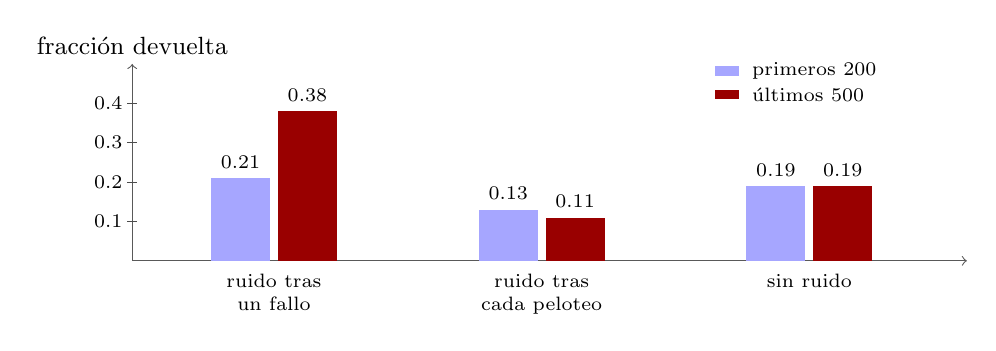
\begin{tikzpicture}[x=1cm,y=5cm]
\draw[->,gray!70!black] (0,0) -- (10.6,0);
\draw[->,gray!70!black] (0,0) -- (0,0.5) node[above,font=\small,black] {fracción devuelta};
\foreach \v in {0.1,0.2,0.3,0.4}{\draw[gray!60!black] (-0.06,\v) -- (0.06,\v); \node[left,font=\scriptsize] at (0,\v) {\v};}
\foreach \x/\f/\l/\lab in {1.8/0.21/0.38/{ruido tras\\un fallo},5.2/0.13/0.11/{ruido tras\\cada peloteo},8.6/0.19/0.19/{sin ruido}}{
  \fill[blue!35] (\x-0.8,0) rectangle (\x-0.05,\f);
  \fill[red!60!black] (\x+0.05,0) rectangle (\x+0.8,\l);
  \node[below,font=\scriptsize,align=center] at (\x,-0.01) {\lab};
  \node[above,font=\scriptsize] at (\x-0.425,\f) {\f};
  \node[above,font=\scriptsize] at (\x+0.425,\l) {\l};}
\fill[blue!35] (7.4,0.47) rectangle (7.7,0.495); \node[right,font=\scriptsize] at (7.75,0.482) {primeros 200};
\fill[red!60!black] (7.4,0.41) rectangle (7.7,0.435); \node[right,font=\scriptsize] at (7.75,0.422) {últimos 500};
\end{tikzpicture}
\caption{Modelo de “revolver tras el fallo” (\texttt{dishbrain\_model.py}): fracción de pelotas devueltas al principio y al final de $2000$ peloteos, promedio de cuarenta cultivos modelo. Solo hay aprendizaje si el empujón sigue al fallo y no al acierto, como en el experimento, donde el aumento significativo en la sesión solo se dio con retroalimentación completa.}
\label{fig:dishmodel}
\end{figure}

\begin{keyblock}
\begin{proposition}[El maestro que revuelve]
\label{prop:dishscramble}
Si el fracaso sacude la red y el éxito la deja en paz, la red deriva por sí sola hacia ajustes que fallan menos: el tiempo pasado en un ajuste es inversamente proporcional a la probabilidad de fracaso~\eqref{eq:dishdensity}. Para este aprendizaje no hacen falta ni una señal de recompensa, ni su signo, ni la predictibilidad como tal: basta con que la retroalimentación tras el éxito y tras el fracaso sea distinta. El cambio de comportamiento del cultivo está medido; qué mecanismo actúa en la placa, predicción de la entrada o revoltura, no está establecido.
\end{proposition}
\end{keyblock}

Compárese con el capítulo~\ref{sec:dofa}. Allí el ruido también servía de búsqueda, pero la dopamina tenía signo: el error $\delta$ decía en qué sentido mover los pesos, y el paso seguía el gradiente~\eqref{eq:perturbation}. Aquí no hay signo: solo “dejar” o “sacudir”. Esta búsqueda es más burda y más lenta, pero le pide menos a la red: ni neuronas \nt{DOPA}, ni crítico, ni una traza que dure segundos.

\section{Qué se midió y qué se discute}

Cada partida duraba $20$ minutos; se comparaban los primeros $5$ minutos con los últimos $15$. En los cultivos con retroalimentación completa, las series de pelotas devueltas se alargaron y los fallos inmediatos disminuyeron; en los controles sin células, sin juego y con una “raqueta” de computadora no pasó nada parecido. Los cultivos de células humanas devolvían en promedio durante más tiempo que los de ratón. La mejora es estadísticamente sólida (en nueve cultivos de ratón y once humanos, con más de un centenar de partidas en cada grupo), pero pequeña: la red no se volvió un buen jugador, se volvió algo mejor que el azar. Es sólida dentro de la sesión; los autores no obtuvieron un aprendizaje estable de una sesión a otra a lo largo de varios días~\cite{Kagan2022}. Un trabajo posterior del mismo grupo encontró que durante el juego la actividad del cultivo se acerca al régimen \emph{crítico}, la frontera entre la extinción y la avalancha, esa misma vida al borde del capítulo~\ref{sec:gaba}, y que cuanto más cerca, mejor el juego~\cite{Habibollahi2023}.

La principal polémica no la causaron las cifras, sino las palabras. El título del artículo afirmaba que las neuronas en la placa “muestran sintiencia” (sentience), y un grupo de investigadores objetó: un cambio de comportamiento en lazo cerrado no es todavía inteligencia ni sensación, y las conclusiones deben formularse con más modestia~\cite{Balci2023}. Desde el punto de vista del ingeniero quedan abiertas dos preguntas, y las dos son sobre el mecanismo. Primera: ¿aprende la red, es decir, cambian sus pesos de forma duradera, o la retroalimentación solo desplaza su estado actual? Segunda: ¿hace falta precisamente la predictibilidad, o basta cualquier diferencia entre la respuesta al éxito y al fracaso, como en la proposición~\ref{prop:dishscramble}? Un banco en el que cada electrodo es accesible permite responder a ambas, y ese es quizá su principal valor.

\section{Especificación del banco: cómo reproducirlo}
\label{sec:dishspec}

A continuación está todo lo necesario para montar de nuevo un banco así: el equipo, el lazo, la codificación de la entrada, la lectura de la salida, la retroalimentación y el protocolo del experimento. Cada parámetro lleva indicada su fuente. “Artículo”: el valor está tomado del texto del trabajo~\cite{Kagan2022}. “Elección”: el artículo no lo da, y para reproducirlo habrá que fijarlo uno mismo; proponemos un valor por defecto y decimos cómo comprobarlo.

\subsection*{Equipo y cultivo}

\begin{center}
\footnotesize
\setlength{\tabcolsep}{4pt}
\renewcommand{\arraystretch}{1.15}
\begin{tabular}{>{\raggedright}p{4.0cm}>{\raggedright}p{6.9cm}>{\raggedright\arraybackslash}p{1.6cm}}
\toprule
Parámetro & Valor & Fuente \\
\midrule
chip & matriz MaxOne: $26\,000$ electrodos de platino en un área de $8$~mm$^2$ & artículo \\
registro & hasta $1024$ canales a la vez, $20\,000$ muestras por segundo & artículo \\
estimulación & técnicamente hasta $32$ electrodos; en el experimento, $8$ independientes & artículo \\
células & corteza de embrión de ratón; neuronas humanas a partir de células madre (dos métodos de cultivo); células HEK293T (no neuronas) como control & artículo \\
siembra & alrededor de $10^6$ células por chip & artículo \\
edad del cultivo en el experimento & ratón: desde $\sim10$ días; humano: $14$--$24$ días o $\sim80$ días según el método de cultivo & artículo \\
\bottomrule
\end{tabular}
\end{center}

\subsection*{Lazo y tiempo}

El lazo funciona en ventanas de $10\ms$ ($200$ muestras): en cada ventana se cuentan las espigas en los electrodos de las regiones motoras, se actualiza el juego y se emite la siguiente estimulación. El retardo desde una espiga en el cultivo hasta el estímulo de respuesta es de unos $5\ms$. Durante el juego, la señal de cada electrodo pasa por un filtro de Bessel paso alto de 2.º orden con frecuencia de corte de $100$~Hz; el valor absoluto de la señal se suaviza con un filtro de Bessel paso bajo de 1.er orden de $1$~Hz, y el umbral de espiga es proporcional a ese valor absoluto suavizado. El umbral de seis desviaciones estándar del fondo el artículo lo indica para mediciones aparte de la actividad, no para el juego. Para que la estimulación no cuente como respuesta del cultivo, todas las señales se anulan cuando llegan a la vez más de $15$ pulsos grandes, de más de $75$~mV. Todo esto: artículo.

\subsection*{Codificación de la pelota}

\begin{center}
\footnotesize
\setlength{\tabcolsep}{4pt}
\renewcommand{\arraystretch}{1.15}
\begin{tabular}{>{\raggedright}p{3.4cm}>{\raggedright}p{7.5cm}>{\raggedright\arraybackslash}p{1.6cm}}
\toprule
Parámetro & Valor & Fuente \\
\midrule
región sensorial & $8$ electrodos dispuestos de modo que electrodos vecinos signifiquen posiciones vecinas de la pelota & artículo \\
código de lugar & el número de electrodo $k=1,\dots,8$ da la posición de la pelota respecto al centro de la raqueta & artículo \\
qué coordenada & la posición vertical de la pelota; para reproducirlo, respecto a la raqueta, $k=\lceil 8(y-p+\tfrac12)\rceil$ con $y-p\in[-\tfrac12,\tfrac12]$ & artículo; fórmula: elección \\
código de frecuencia & una frecuencia de estimulación de $4$ a $40$~pulsos/s lleva la distancia a la raqueta & artículo \\
sentido de la escala & $4$~pulsos/s cuando la pelota está junto a la pared opuesta, y linealmente hasta $40$~pulsos/s cuando está junto a la pared de la raqueta: $f=4+36\,(1-x/L)$, $x$ es la distancia a la pared de la raqueta, $L$ el ancho de la cancha & artículo \\
forma del pulso & rectangular bifásico corto: primero la fase positiva, luego la negativa & artículo \\
amplitud & $75$~mV; elegida para no forzar el disparo de las células inhibidas & artículo \\
duración de las fases & no indicada; usar el ajuste estándar del sistema de estimulación y no cambiarlo durante el experimento & elección \\
\bottomrule
\end{tabular}
\end{center}

\subsection*{Lectura de la raqueta}

En el artículo hay dos regiones motoras: las espigas en la primera mueven la raqueta hacia arriba; en la segunda, hacia abajo. La contribución de las regiones se pondera para tener en cuenta su distinta densidad de células y su distinta actividad~\cite{Kagan2022}. La fórmula exacta no se da. Para reproducirlo tomamos la regla~\eqref{eq:dishreadout}, $\Delta p=c\,(n_\uparrow-n_\downarrow)$ en cada ventana de $10\ms$, con un peso que iguala las regiones por su actividad media en reposo (elección): $n_\uparrow$ y $n_\downarrow$ se dividen entre la cuenta media de su región por ventana, medida antes del juego. El coeficiente $c$ se elige de modo que una diferencia de una cuenta media desplace la raqueta un $1\%$ de la altura de la cancha por ventana (elección); así, un predominio constante de una región lleva la raqueta de un lado a otro de la cancha en $1$~s.

La ubicación de las regiones en el chip no está dada con coordenadas en el texto del artículo; solo hay un esquema. Para reproducirlo bastan tres grupos de electrodos disjuntos: los ocho sensoriales en el centro y un grupo de electrodos de registro a cada lado, uno “arriba” y otro “abajo” (elección).

\subsection*{El juego}

El tamaño de la cancha, la longitud de la raqueta y la velocidad de la pelota no se indican en el artículo; solo se dice que la pelota vuela a velocidad constante y rebota en las paredes. Para reproducirlo (elección): cancha de $1\times1$, raqueta de longitud $0.2$ en la pared derecha (acierto con $|y-p|<0.1$, como en el modelo~\texttt{models/dishbrain\_model.py}), y la pelota cruza la cancha en $1$~s. Un fallo sin ninguna pelota devuelta en el peloteo cuenta como “ace”; un peloteo de más de tres golpes seguidos, como “largo” (artículo).

\subsection*{Retroalimentación}

\begin{center}
\footnotesize
\setlength{\tabcolsep}{4pt}
\renewcommand{\arraystretch}{1.15}
\begin{tabular}{>{\raggedright}p{2.6cm}>{\raggedright}p{8.3cm}>{\raggedright\arraybackslash}p{1.6cm}}
\toprule
Evento & Qué se aplica & Fuente \\
\midrule
acierto & estímulo predecible: los $8$ electrodos sensoriales a la vez, $75$~mV, $100$~pulsos/s, $100\ms$; la estimulación normal de la pelota se interrumpe durante ese tiempo & artículo \\
fallo & estímulo impredecible: $150$~mV, $5$~pulsos/s, $4$~s, en instantes aleatorios y en electrodos elegidos al azar entre los $8$; luego $4$~s sin estimulación, y la pelota sale en una dirección aleatoria & artículo \\
ley del azar & no indicada; para reproducirlo, los instantes de los pulsos como un proceso de Poisson de frecuencia media $5$~pulsos/s & elección \\
\bottomrule
\end{tabular}
\end{center}

\subsection*{Protocolo y control}

Una sesión dura $20$~min; se comparan los primeros $5$ y los últimos $15$~min (artículo). Tres medidas del resultado: la longitud media del peloteo, la fracción de aces y la fracción de peloteos largos. Condiciones del experimento (artículo):
\begin{itemize}
\item \emph{estímulo}: el lazo completo, como se describe arriba;
\item \emph{silencio}: en lugar del estímulo de acierto o de fallo, el mismo tiempo sin ninguna estimulación; luego la pelota sale en una dirección aleatoria;
\item \emph{sin retroalimentación}: tras un fallo la pelota simplemente rebota y sigue volando, y la estimulación de la posición de la pelota continúa;
\item \emph{reposo}: el juego sigue y la raqueta se mueve según la actividad, pero no hay ninguna estimulación;
\item \emph{controles}: chip solo con medio; células HEK293T; “cultivo en la computadora”, una simulación en lugar de células.
\end{itemize}
Tamaño de muestra en la serie principal: $9$ cultivos de ratón ($101$ sesiones), $11$ cultivos humanos ($138$), $6$ chips con medio ($80$), $20$ cultivos en reposo ($42$), $3$ simulaciones ($38$); en total, $399$ sesiones. En la serie sobre la retroalimentación: $486$ sesiones en $3$ días, $3$ sesiones al día, con las condiciones “estímulo”, “silencio” y “sin retroalimentación” ($n=27$, $17$ y $15$). El aumento de la longitud media del peloteo de los primeros $5$ minutos a los últimos $15$ solo se obtuvo en cultivos vivos. En la serie sobre la retroalimentación, el aumento significativo en el tiempo solo se dio en la condición “estímulo”; al final de la sesión la condición “silencio” sí superaba a “sin retroalimentación”, pero con un efecto menor, y no hubo aprendizaje estable de una sesión a otra en los tres días~\cite{Kagan2022}.

\subsection*{El ciclo del banco paso a paso}

Cada $10\ms$ la computadora del banco hace lo siguiente.
\begin{enumerate}
\item Lee el número de espigas $n_\uparrow$, $n_\downarrow$ en las dos regiones motoras durante la ventana anterior y lo normaliza por la cuenta media de la región en reposo.
\item Desplaza la raqueta en $\Delta p=c\,(n_\uparrow-n_\downarrow)$ y la limita a los bordes de la cancha.
\item Avanza la pelota un paso; la hace rebotar en las paredes superior, inferior e izquierda.
\item Si la pelota llegó a la pared derecha: con $|y-p|<0.1$ hay acierto, la cuenta del peloteo sube en uno y se aplica el estímulo de acierto ($100\ms$); si no, hay fallo, se registra el peloteo, se aplica el estímulo de fallo ($4$~s), luego $4$~s de pausa, y la pelota vuelve a salir.
\item Si no, elige el electrodo $k$ según la posición vertical de la pelota y la frecuencia $f$ según la distancia a la pared de la raqueta, y aplica al electrodo $k$ pulsos bifásicos de $75$~mV con frecuencia $f$ hasta la siguiente ventana.
\end{enumerate}
Esto basta para montar un banco compatible con el publicado y comprobar la pregunta principal del capítulo: si al cultivo le enseña la predictibilidad o la simple diferencia entre la respuesta al acierto y al fallo. Para ello conviene añadir a las tres condiciones del artículo una cuarta que no está en él: tras el fallo, un estímulo \emph{predecible} de la misma duración y energía que el impredecible. Si el cultivo aprende también así, lo que cuenta es la diferencia, no la predictibilidad.


\section{Resumen}

\begin{table}[t]
\centering
\footnotesize
\setlength{\tabcolsep}{4pt}
\renewcommand{\arraystretch}{1.15}
\begin{tabular}{>{\raggedright}p{2.1cm}>{\raggedright}p{4.2cm}>{\raggedright}p{1.9cm}>{\raggedright\arraybackslash}p{4.6cm}}
\toprule
Bloque del banco & Cómo está hecho & Capítulo del libro & Qué se sabe \\
\midrule
entrada & lugar (cuál de los 8 electrodos) y frecuencia (4--40 pulsos/s) & \ref{sec:code}, \ref{sec:sensors} & lo fija el experimentador \\
salida & diferencia de cuentas de dos regiones en $10\ms$~\eqref{eq:dishreadout} & \ref{sec:glutcomputer}, \ref{sec:debugging} & lo fija el experimentador; ruido según~\eqref{eq:rateerror} \\
maestro & estímulo predecible tras el acierto, impredecible tras el fallo; sin dopamina & \ref{sec:dofa} & aumento significativo en la sesión solo con retroalimentación completa; con silencio el efecto es menor; inestable de una sesión a otra \\
mecanismo & predicción de la entrada o revoltura tras el fallo~\eqref{eq:dishdensity} & \ref{sec:dofa}, \ref{sec:recognition} & no establecido; ambos explican el resultado \\
régimen de la red & acercamiento al régimen crítico durante el juego & \ref{sec:gaba} & la relación con la calidad del juego está medida \\
“sintiencia” & afirmación de los autores & --- & no demostrada; discutida \\
\bottomrule
\end{tabular}
\caption{DishBrain visto por un ingeniero.}
\label{tab:dishbrain}
\end{table}

DishBrain es una máquina de neuronas vivas en su forma más simple: la entrada está dada por un código, la salida se lee con una cuenta, y el maestro es la diferencia entre la respuesta al éxito y al fracaso (tabla~\ref{tab:dishbrain}). Una red sin ojos, músculos ni dopamina aprendió a jugar un poquito, y ya eso la convierte en un banco de pruebas para las ideas del libro. Sea cual sea el mecanismo (predicción, revoltura o una tercera cosa), la respuesta se encontrará como aconseja el capítulo~\ref{sec:debugging}: con la sonda, la señal de prueba y la desconexión de partes, en una máquina que por fin se ve entera.

\section{Ejercicios}

\begin{exercise}[\lvlA]
\label{ex:22:1}
\emph{Cuánto hay que desplazar la cuenta.} Las dos regiones emiten juntas $R_\uparrow+R_\downarrow=2000$ espigas/s (Poisson). (a)~¿Dispersión relativa de la cuenta de una región en $10\ms$ con $R=1000$ y $R=100$? (b)~En $1$~s de vuelo de la pelota los desplazamientos~\eqref{eq:dishreadout} se suman. ¿Con qué $R_\uparrow-R_\downarrow$ mínima el desplazamiento medio duplica la dispersión?
\end{exercise}

\begin{exercise}[\lvlA]
\label{ex:22:2}
\emph{Cuántos peloteos hacen falta para ver el aprendizaje.} Los peloteos son independientes y la fracción devuelta es binomial. ¿Cuántos peloteos hacen falta en cada uno de dos periodos para que el aumento de la fracción devuelta supere dos desviaciones estándar de la diferencia: (a)~de $0.20$ a $0.25$; (b)~de $0.21$ a $0.38$, como en el modelo?
\end{exercise}

\begin{exercise}[\lvlB]
\label{ex:22:3}
\emph{Deducción de~\eqref{eq:dishdensity}.} El ajuste $\boldsymbol\psi$ recorre un conjunto finito; tras un fallo (probabilidad $P(\boldsymbol\psi)>0$) la red pasa a $\boldsymbol\psi'$ con probabilidad simétrica $K(\boldsymbol\psi,\boldsymbol\psi')$, y tras un acierto se queda. (a)~Demuestre que $\rho\propto1/P$ es la distribución estacionaria. (b)~¿Cuál es la fracción de fallos con dos ajustes de $P=0.9$ y $P=0.1$?
\end{exercise}

\begin{exercise}[\lvlB]
\label{ex:22:4}
\emph{La región absorbente del modelo.} La raqueta llega a $p=\min\bigl(1,\max(0,ay+b)\bigr)$, la pelota a la altura $y\sim U(0,1)$, y hay acierto si $|p-y|<h=0.1$. (a)~Demuestre que con $|b|<h$ y $|a-1+b|<h$ la red devuelve todas las pelotas, y halle el área de esta región. (b)~Halle numéricamente la fracción media devuelta con $a\sim U(-1,1)$, $b\sim U(0,1)$.
\end{exercise}

\begin{exercise}[\lvlB]
\label{ex:22:5}
\emph{Simulación: una valla alrededor de los ajustes.} En una copia de \texttt{dishbrain\_model.py}, dé a $200$ cultivos $20\,000$ peloteos a cada uno. ¿Cuál es la fracción devuelta en los últimos $500$? ¿Y si tras cada empujón se recorta el ajuste al rectángulo $a\in[-1,2]$, $b\in[-1,1]$? Explique la diferencia con ayuda del ejercicio~\ref{ex:22:3}.
\end{exercise}

\begin{exercise}[\lvlB]
\label{ex:22:6}
\emph{Diseño del código de entrada.} La pelota se devuelve si el error en altura es menor que $h=0.1$; la red lee la entrada en $T=0.25$~s, hasta la frecuencia $r$ distingue unos $\sqrt{rT}$ niveles, y la estimulación no pasa de $40$ pulsos/s. (a)~¿Basta un código de lugar con ocho electrodos? (b)~¿Y la altura por frecuencia en un solo electrodo?
\end{exercise}

\begin{exercise}[\lvlC]
\label{ex:22:7}
\emph{Investigación: ¿predicción o revoltura?} Generalice el modelo a $d$ números ajustables ($p=\sum_{i<d}a_iy^i$). ¿Cómo crece con $d$ el número de peloteos hasta una fracción devuelta de $0.5$ con revoltura y con la regla con signo del error~\eqref{eq:perturbation}? ¿Qué experimento en el banco separaría las dos hipótesis?
\end{exercise}
